\documentclass[a4paper,12pt]{article}

\usepackage{cmap}		
\usepackage[utf8]{inputenc}			
\usepackage[english,russian]{babel}
\usepackage{framed}
\usepackage{hyperref}
\usepackage{amsmath}
\usepackage[colorinlistoftodos]{todonotes}
\usepackage{wrapfig}
\usepackage{lipsum}
\usepackage{listings}
\usepackage{color}
\usepackage{indentfirst}
\usepackage{times}
\usepackage{textcomp}
\usepackage{smartdiagram}
\usepackage{caption}
\usesmartdiagramlibrary{additions}
\usepackage{tikz}
\usepackage{multicol}
\usepackage{lipsum}
\usepackage{mwe}
\usepackage{floatrow}
\usepackage[ruled,linesnumbered,vlined]{algorithm2e}
\usepackage{algpseudocode}
% \usepackage[final]{graphicx}
\usepackage{subfigure}
\usepackage{subcaption}
\usepackage{minted}
\usepackage{placeins}
\usepackage{amsfonts}
\usepackage{lscape}
\usepackage{subcaption}
\usepackage{enumitem}
\usepackage{siunitx}
\usepackage{array}
\usepackage{pgfplots}
\pgfplotsset{compat=newest}
\usetikzlibrary{arrows,shapes}
\DeclareMathOperator*{\argmin}{arg\,min}
\DeclareMathOperator*{\argmax}{arg\,max}
\DeclareMathOperator{\E}{\mathbb{E}}
\definecolor{deepblue}{rgb}{0,0,0.5}
\definecolor{deepred}{rgb}{0.6,0,0}
\definecolor{deepgreen}{rgb}{0,0.5,0}

\newcommand{\HRule}{\rule{\linewidth}{0.5mm}}
\DeclareMathOperator*{\argmax}{arg\,max}
\DeclareMathOperator*{\argmin}{arg\,min}

% Default fixed font does not support bold face
\DeclareFixedFont{\ttb}{T1}{txtt}{bx}{n}{12} % for bold
\DeclareFixedFont{\ttm}{T1}{txtt}{m}{n}{12}  % for normal


% Python style for highlighting
\newcommand\pythonstyle{\lstset{
language=Python,
basicstyle=\ttm,
otherkeywords={self},             % Add keywords here
keywordstyle=\ttb\color{deepblue},
emph={MyClass,__init__},          % Custom highlighting
emphstyle=\ttb\color{deepred},    % Custom highlighting style
stringstyle=\color{deepgreen},
frame=tb,                         % Any extra options here
showstringspaces=false            % 
}}


% Python environment
\lstnewenvironment{python}[1][]
{
\pythonstyle
\lstset{#1}
}
{}

% Python for external files
\newcommand\pythonexternal[2][]{{
\pythonstyle
\lstinputlisting[#1]{#2}}}

% Python for inline
\newcommand\pythoninline[1]{{\pythonstyle\lstinline!#1!}}

\begin{document}

\begin{titlepage}
\begin{center}

\textsc{\Large Московский Государственный Технический Университет имени Н.Э.Баумана}\\
\textsc{\large (Национальный Исследовательский Университет)}\\[1.5cm]

% Upper part of the page. The '~' is needed because \\
% only works if a paragraph has started.

\includegraphics[width=0.3\textwidth]{img/logo.png}~\\[1cm]

\textsc{\Large Курсовой проект по проектированию}\\[0.5cm]

% Title
\HRule \\[0.4cm]
{ \LARGE \bfseries Проектирования системы управления на базе обучения с подкреплением\\[0.4cm] }

\HRule \\[1.5cm]

% Author and supervisor
\noindent
\begin{minipage}{0.4\textwidth}
\begin{flushleft} \large
\emph{Студент:}\\
Юнес \textsc{А.~Ю.}
\end{flushleft}
\end{minipage}%
\begin{minipage}{0.4\textwidth}
\begin{flushright} \large
\emph{Рукаводитель:} \\
Ющенко \textsc{А.~С.}
\end{flushright}
\end{minipage}

\vfill

% Bottom of the page
{\large \today}

\end{center}
\end{titlepage}

% \newpage
% \begin{abstract}
    
%     The standard control methods in robotics are based on the dynamical model of the robot, and also on the model of the dynamics of the environment to build the needed closed loop control scheme; in the real world to realize such methods for manipulators, we have to follow the following steps: (1) taking an observation of the environment using cameras or sensors (2) estimating the state of the robot and the task (e.g,position of the end-effector and the goal position) (3) planing the trajectory of motion of the end-effector to achieve the task (4) using low-level controllers (or force controller for harder tasks) to ensure following the planned path by minimizing the errors (5) sending the resulting commands to the joints of the robot. The errors which are occurred in each step, accumulated to produce a cumulative error making the control process hard to realize with desired accuracy.\\ \par
%     We suggest using the machine learning to achieve end-to-end mapping directly from observations to joints' motors commands, exploit the last deep learning revolution in using deep (large) neural networks. The state of the art deep reinforcement learning algorithms, that tried to handle robotic tasks can be classified to two major classes: (1) model-free algorithms: (like TRPO,PPO,DDPG) which can learn to achieve the task after sampling training sets from interacting with environment, so we can consider the robot's model as a black-box (2)model-based algorithms: depends on a known (or learned) transition model of the environment. The model-free algorithms need days of training to learn basic robotic tasks. On the other hand, model-based algorithms can learn much more faster (less than an hour), but can't adapt to unforeseen situation (the learned model is no longer valid).\\ \par
%     We intend in that research to develop a data-efficient model-free algorithm, which can get the benefits of the both classes of deep reinforcement learning algorithms, and learn the assembly task (which is considered as a hard problem in standard robotic control) in a considerable small period of time.
% \end{abstract}
\newpage
\tableofcontents

\newpage
\listoffigures
\listoftables
 
\newpage
\section{Введение}
\subsection{Обучения с подкреплением - от игр к промышленности}
Целью машинного обучения является частичная или полная создания машину, способную учиться аналогично человеку. Основные стандартные типы задач машинного обучения; (1) Обучение с учителем , при котором машина обучается на основе помеченных данных. (2) Обучение без учителя , процесс обучения работает с непомеченными данными и (3) Обучение с подкреплением, когда процесс обучения зависит от проб и ошибок.\\

Технологические достижения последних лет привели к использованию глубоких нейронных сетей в алгоритмах обучения в качестве мозга машины. Забота о лучших способах мышления вызвала некоторые идеи на свет - одной из них было обучение с подкреплением. Глубокое обучение с подкреплением стала трендом, и базом "Искусственного общего интеллекта" (Artificial General Intelligence).\\

В 2015 году команда Google DeepMind опубликовала статью в журнале Nature, представляющую систему, основанную на обучении подкреплению, под названием AlphGO. Эта система победила над чемпионатом мира в игре GO. Такие важный достижения, мотивировала многих исследователей следовать этому направлению исследований. Новые алгоритмы разработаны после этого, сформировали революцию в приложениях обучения с подкреплением.\\
\begin{figure}[H]
    \centering
    \subfigure[Машинное обучение]{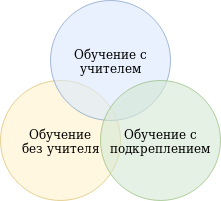
\includegraphics[height=5cm]{img/ML.png}}
    \subfigure[AlphaGO]{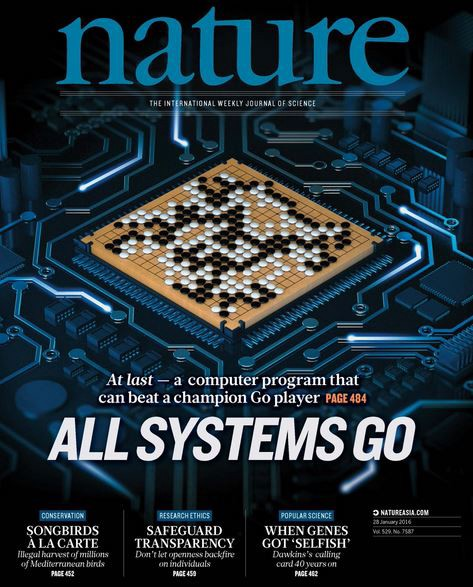
\includegraphics[height=5cm]{img/go.jpeg}}
    \caption{Обучения с подкреплением - от игр к промышленности}
    \label{fig:my_label}
\end{figure}

Но два года позже, в 2017. Опубликовали статью под названием «Глубокое обучение с подкреплением пока не работает», в котором представлен обзор и результаты современных алгоритмов глубокого обучение с подкреплением. Эта статья показала, что еще много работы, чтобы иметь идеальный вариант из алгоритмов обучения с подкреплением.\\

В промышленности интерес заключается в оптимизации процессов производства при сохранении некоторых строгих ограничений. Обучения с подкреплением показало, что он может превзойти человеку и классической управление, когда он работает, поэтому наша цель в этой работе - исследовать различные алгоритмы обучения с подкреплением и обсудить, как мы можем заставить обучение с подкреплением чтобы работать хорошо в реальных промышленных задачах. Попытался предложить практические решения на основе  обучения с подкреплением.\\

\subsection{Актуальность и важность обучения в робототехники}
В области промышленности и робототехники у нас могут быть дополнительные требования к системе наряду с выполнением ее задач. Например, если система космического аппарата с управлением соответствует ракетным двигателям, то целью является достижение Луны с минимальным расходом топлива. 
Оптимальное управление решает такие задачи, ставя своей целью найти закон управления для динамической системы за такой промежуток времени, чтобы целевая функция была оптимизирована; определение набора дифференциальных уравнений, описывающих путь управляющих переменных, которые минимизируют функцию затрат.\\

Модельное прогнозирующее управление (Model predictive control MPC) является одним из популярных методов оптимального управления. MPC был разработан в обществе системы управления, в общем он обеспечивает стабильности, осуществимость и надежности. Кроме того, он может обрабатывать ограничения на систему. Но он основан на динамической модели системы, поэтому на него влияет точность этой модели, и он не может адаптироваться к изменениям и требует высокая вычислительная сложность.\\

С другой стороны, обучение с подкреплением (которое также можно рассматривать как часть оптимального управления) не зависит от модели, способно адаптироваться и имеет низкую вычислительную сложность при развертывании модели после обучения. Но он обладает незрелой стабильностью, осуществимостью и надежностью и трудно обрабатывать ограничения.\\

Мы можем ясно заметить комплементарную связь между модельным прогностическим контролем MPC и обучением с подкреплением, Мы будем в этой работе исследовать, как мы могли бы использовать преимущества обеих парадигм, чтобы получить наилучшие результаты в решении задач управления.

\begin{table}[H]
    \centering
    \captionsetup{justification=centering,margin=1cm}
    \begin{tabular}{| >{\centering\arraybackslash\hspace{0pt}}m{2cm}| >{\centering\arraybackslash\hspace{0pt}}m{5cm}| >{\centering\arraybackslash\hspace{0pt}}m{5cm}|}
         \hline
         Свойство & Модельное прогнозирующее управление & Обучение с подкреплением\\
         \hline
         Модель & Требуемый (-) & Не Требуемый (+)\\
         \hline
         Адаптивность & Зависит от надежность (-) & Присущий (+)\\
         \hline
         Онлайн выч. сложность & Высокая (-)& Низкая (+)\\
         \hline
         Офлайн выч. сложность & Низкая (+) & Высокая (-) \\
         \hline
         Стабильность & Зависит от терминального стоимости (+) & Неприсущий(-) \\
         \hline
         Осуществимость & Зависит от терминального ограничения (+) & Неприсущий(-) \\
         \hline
         Надежностью & Присущий (+) & Неприсущий(-) \\
         \hline
         Обработка ограничений & Присущий (+) & Неприсущий(-) \\
         \hline
    \end{tabular}
    \caption{Сравнения  Модельного прогнозирующего управления с Обучением с подкреплением}
    \label{tab:my_label}
\end{table}
\newpage
\section{Постановка задачи}
В обычной модели прогностического регулятора MPC целью является нахождение оптимального управления путем решения задачи оптимизации (оптимизации целевого функционала) по горизонту времени, используя данный модель динамической системы.\\

Мы заинтересованы в использовании модели прогностического управления MPC , когда у нас нет динамической модели системы, а мы будем обучать модель и планировать в ней.\\

Вместо обучения динамическую модель явно, мы будем рассматривать систему как систему Марковского процесса принятия решений (аналогично случаю в обучении подкреплению).\\

Полный алгоритм можно рассматривать как основанную на модели задачу обучения с подкреплением, с моделью прогностического регулятора в качестве планировщика. Или проблема модели прогностического управления на основе обучения с подкреплением.\\

\begin{figure}[H]
    \centering
    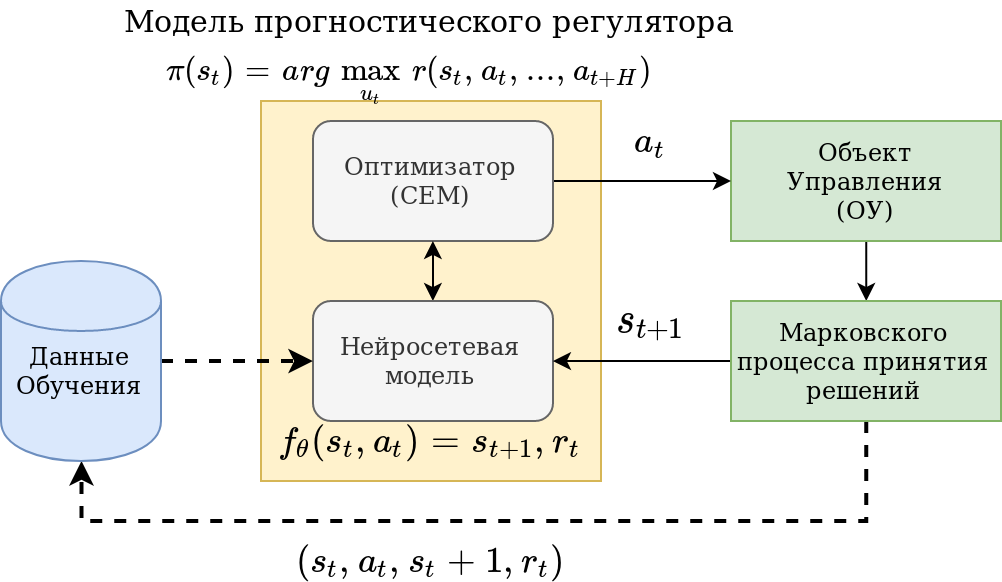
\includegraphics[height=8.5cm]{img/mpc_ru.png}
    \caption{MPC на основе обучения с подкреплением}
    \label{fig:my_label}
\end{figure}
\newpage
Мы протестируем наш прототип на двух основных средах:
\begin{enumerate}[noitemsep]
    \item Маятник на тележке (Cart Pole):\\
Маятник на тележке - общий эталонный тест для алгоритмов управления и обучения с подкреплением, маятник прикреплен неуправляемым маятник к тележке, которая движется по пути без трения. Система управляется путем приложения силы +1 или -1 к тележке. Маятник начинает двигаться вертикально, и цель состоит в том, чтобы предотвратить его падение. Вознаграждение в размере +1 предоставляется за каждый шаг времени, когда маятник остается в вертикальном положении.
\begin{figure}[H]
    \centering
    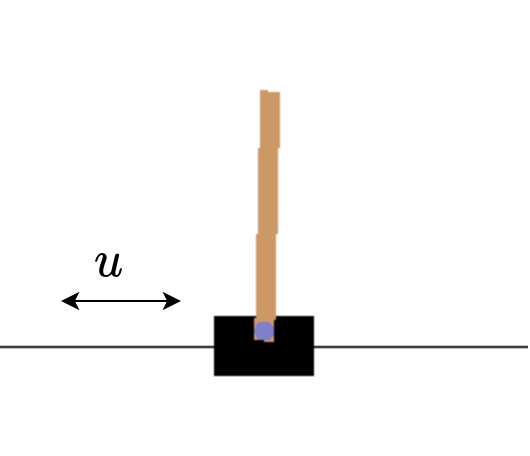
\includegraphics[height=3cm,trim={0 2cm 0 2cm},clip]{img/cart.png}
    \caption{Маятник на тележке (Cart Pole)}
    \label{fig:my_label}
\end{figure}
\item Манипулятор 7 степень свободы:\\
Позиция цели выбирается случайным образом в 3D пространстве. Мы должны управлять манипулятор, чтобы достичь этой цели как можно быстрее. Манипулятор управляется в пространстве шарниров т. е. каждое действие состоит из 7 команд относительного движения к двигателям шарниров. Вознаграждение дается как отрицательное расстояние до цели.
\begin{figure}[H]
    \centering
    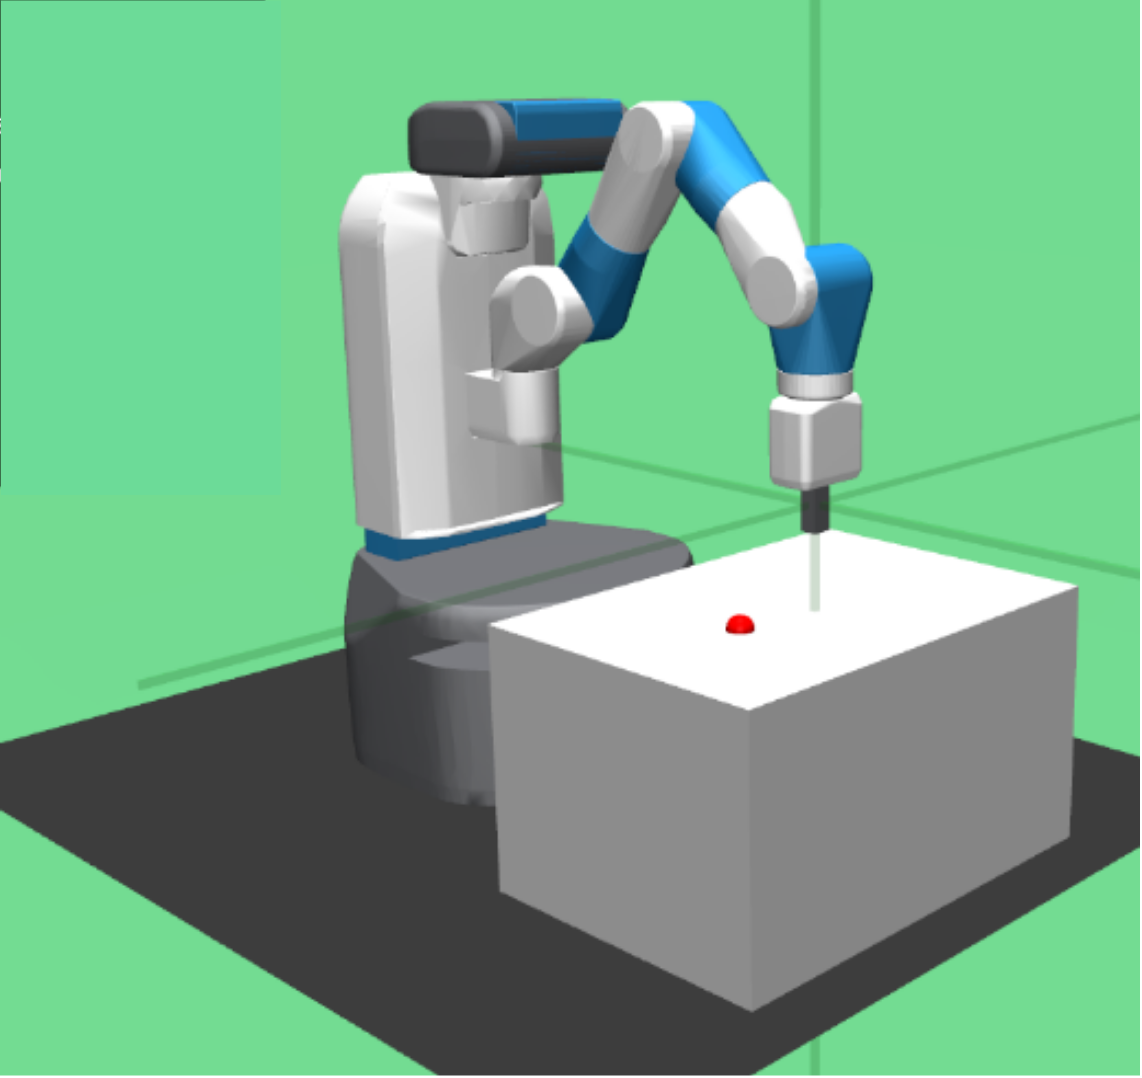
\includegraphics[height=6cm,trim={0 2cm 0 2cm},clip]{img/arm.png}
    \caption{Манипулятор 7 степень свободы}
    \label{fig:my_label}
\end{figure}

\newpage
\end{enumerate}
\section{Исследовательская часть} 
\subsection{Оптимальное управления}
\subsubsection{Модель системы и функция стоимости:}
рассмотрим дискретной линейной стационарной системы
\begin{equation}
    x(t+1)=Ax(t)+Bu(t)
\end{equation}
где $x \in \mathbb{R}^n$-вектор состояния, $u \in \mathbb{R}^m$-входной управляющий вектор, $A \in \mathbb{R}^{n \times n}$-системная матрица, $B \in \mathbb{R}^{n \times m}$-входная матрица, $t \in \mathbb{N}$-дискретное время. A и B считаются стабилизированными.\\

Пусть $x(t)$ будет вектор состояния, измеренная в момент времени $t$ и $x_{t+k}$ вектора состояния предсказан в дискретном времени $t+k$, используя уравнение состояния (1) с начальным условием $x_t=x(t)$.//

$x(t)$ и $u(t)$ ограничены из многогранных множеств.\\

Рассмотрим функциал стоимости:
\begin{equation}
    V_N(x(t))=r_T(x_{t+N},u_{t+N})+\sum_{k=0}^{N-1} \gamma^k r(x_{t+k},u_{t+k})
\end{equation}
с стоимость шага:
$$r(x_{t+k},u_{t+k})=x_{t+k}^k Q x_{t+k} + u_{t+k}^T R u_{t+k}$$
и терминальная стоимость:
$$r(x_{t+N},u_{t+N})=x_{t+k}^k P x_{t+k}$$
где $N$-горизонт прогнозирования, $\gamma$-коэффициент дисконтирования,$Q$ состояние весовой матрицы, $R$ входной весовой матрицы и $P$ терминал весовой матрицы.\\

Терминальные матрицы считаются симметричными и положительно определенными.
В качестве решения алгебраического уравнения Риккати выбрана терминальная весовая матрица:
\begin{equation}
    (A+BK)^T P (A+BK)-P+Q+K^T R K=0
\end{equation}
причем :
$$K=-(R+B^T P B)^{-1} B^T P A$$
\subsubsection{Задача Оптимального Управления Конечным Горизонтом}
Оптимизация Функциала:
\begin{equation}
    U_{N}^*(x(t))=\argmin_{U(t)} r_T(x_{t+N},u_{t+N})+\sum_{k=0}^{N-1} \gamma^k r(x_{t+k},u_{t+k})
\end{equation}

\begin{subequations}
C ограничениями:
\begin{align}
    x_{t+k+1} & = Ax_{t+k}+Bu_{t+k}  & k&=0,..,N-1 \\
    x_{t+k} & \in \mathbb{X}  & k&=0,..,N \\
    u_{t+k} & \in \mathbb{U}  & k&=0,..,N-1 \\
    x_t&=x(t) \\
    U(t)&=(u_t^T, ... , u_{t+N-1}^T)^T \in \mathbb{R}^{N_m}
\end{align}
\end{subequations}
Где (5a)- уравнения системы, (5b) - ограничения состоянии, \\ 
\null \qquad (5c) - ограничения управления, (5d) - начальная условия, \\ 
\null \qquad (5e) - управляющая последовательность
\subsubsection{Задача Оптимального Управления Бесконечным Горизонтом}
Оптимизация Функциала:
\begin{equation}
    U_\infty^*(x(t))=\argmin_{U(t)} \sum_{k=0}^{\infty} \gamma^k r(x_{t+k},u_{t+k})
\end{equation}
\begin{subequations}
C ограничениями:
\begin{align}
    x_{t+k+1} & = Ax_{t+k}+Bu_{t+k}  & k&=0,1,.. \\
    x_{t+k} & \in \mathbb{X}  & k&=0,1,.. \\
    u_{t+k} & \in \mathbb{U}  & k&=0,1,.. \\
    x_t&=x(t) \\
    U(t)&=(u_t^T, u_{t+1}^T, ....)^T
\end{align}
\end{subequations}
Где (7a)- уравнения системы, (7b) - ограничения состоянии, \\ 
\null \qquad (7c) - ограничения управления, (7d) - начальная условия, \\ 
\null \qquad (7e) - управляющая последовательность
\newpage
\subsection{Модельное прогнозирующее управление\\
Model Predictive Control (MPC)}
Модельное прогнозирующее управление основано на решении задачи оптимального управления (конечным или бесконечным горизонтом) для измеряемого вектора состояния $x (t)$ с целью получения оптимальной управляющей последовательности $U(t)$ и применения первого элемента оптимальной управляющей последовательности $u(t)=[I,0,..,0] U(t)$ к системе.\\
Эта операция повторяется на каждом дискретном временном шаге t с отступающим горизонтом прогнозирования.\\
\begin{figure}[H]
    \centering
    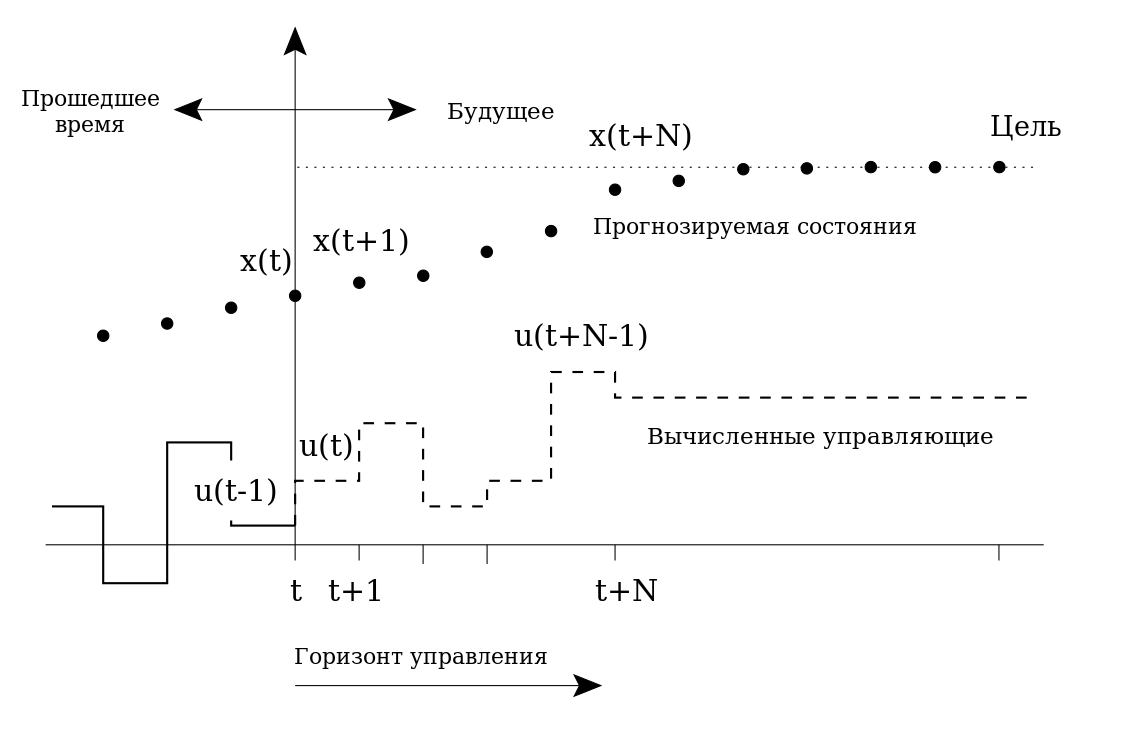
\includegraphics[width=\textwidth]{img/mpc_diag(1).png}
    \caption{Принцип работы модельного прогнозирующего управления}
    \label{fig:my_label}
\end{figure}

Тогда, модельный прогностический контроллер определяется:
\begin{enumerate}
    \item Целовой функционал, которой сведен к минимуму.
\item Внутренняя модель системы для прогнозирования поведения системы.
\item ограничения, которые должны быть удовлетворены.
\end{enumerate}
\newpage
И модельный прогностический регулятор работает в соответствии с следующем:
\begin{enumerate}[noitemsep]
    \item решить задачу оптимизации для вычисления минимума целевого функционала.
\item  Получить последовательность запланированных сигналов управления.
\item  Применить первый управляющий сигнал.
\item  Повторить процедуру планирования.
\end{enumerate}

\subsection{Модельное прогнозирующее управление на основе \\
обучения (Learning-based model predictive control)}
Традиционная модельного прогностического управления опирается на заданном динамическом модели системы и решает задачу оптимизации оптимального управления с ограничениями (уравнение 4,5,6,7).\\

Затем, если динамическая модель недоступна или не точна, эффективность модельного предсказательного регулятора модели будет затронута, и результаты не будут оптимальными.
Обучение может быть использовано для повышения эффективности моделного прогнозного управления, путем (1) обучения остаточной части в качестве коррекции модели, или (2) обучения всей модели на данных, собранных из взаимодействия на реальном управляющем объекте.\\

Мы заинтересованы во втором выборе (2), чтобы в полной мере использовать обучение.
Для того чтобы сформулировать обучающую систему модельного прогностического управления , мы должны выбрать (1) Как мы будем описать обучающей среды (2) Обучаемую модель (3) метод оптимизации. И потом формировать целый цикл управления.\\

В этой работе мы выбрали следующее:\\
(1) Мы определим среду как среду обучения с подкреплением (Марковский процесс принятия решений).\\
(2) Базовой моделью будет нейронная сеть, но чтобы справиться с неопределенностью в модели, мы попытаемся в будущем использовать ансамбль нейронных сетей.\\
(3) Поскольку информация о целевой функции системы непрактична для получения, мы будем использовать оптимизация без производных, в этой работе мы выбрали использовать оптимизатор максимизации перекрестной энтропии.


\newpage
\subsection{Обучения с подкреплением}
Обучение с подкреплением, идея которого была произведена от психологии, является подразделом машинного обучения, изучающим, как агент должен действовать в окружении, чтобы максимизировать некоторый долговременный выигрыш. 

\begin{figure}[H]
    \centering
    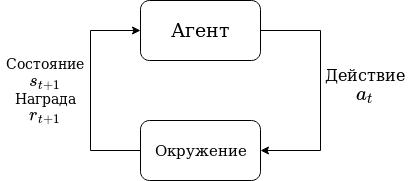
\includegraphics[height=5cm]{img/RL_ru.png}
    \caption{Обучение с подкреплением}
    \label{fig:my_label}
\end{figure}

Окружение обычно формулируется как марковский процесс принятия решений (МППР) с конечным множеством состояний, и в этом смысле алгоритмы обучения с подкреплением связаны с динамическим программированием. Вероятности выигрышей и перехода состояний в МППР обычно являются величинами случайными, но стационарными в рамках задачи.
\begin{center}
\captionof{figure}{марковский процесс принятия решений}
 \begin{tikzpicture}[->, >=stealth', auto, thick, node distance=3cm]

    \tikzstyle{round}=[thick,draw=black,circle]

    \node[round] (s0) {$s_0$};
    \node[round,right= 25mm of s0] (s1) {$s_1$};
    \node[round,above right=7mm and 10mm of s0] (a1){$a_1$};
    \node[round,right= 25mm of s1] (s2) {$s_2$};
    \node[round,above right=7mm and 10mm of s1] (a2){$a_2$};
    \node[round,above right=7mm and 10mm of s2] (a3){$a_3$};

    \path (s0) edge node[below] {$p(s_{t+1}|s_t,a_t)$}(s1)
          (s0) edge node {$\pi_\theta$} (a1)
          (a1) edge node {} (s1);
    \path (s1) edge node[below] {$p(s_{t+1}|s_t,a_t)$}(s2)
          (s1) edge node {$\pi_\theta$} (a2)
          (a2) edge node {} (s2);
    \path (s2) edge node {$\pi_\theta$} (a3);
\end{tikzpicture}
\end{center}
Где $s_t$ - состояние, $a_t$ действие, $r_t$ Награда  \\
Вероятность перехода : $p(s_{t+1}|s_t,a_t)$ \\
Функция стратегии: которая дает наилучшее действие для каждого состояния после процесса обучения: $a \sim \pi_\theta (a_t|s_t)$\\
Цель состоит в том, чтобы максимировать ожидаемые долгосрочные выгрриш:
$$J (\theta)=\sum_{t=1}^{T} \mathbb{E} [r (s_t), \theta]$$
\newpage
\subsection{Обучение с подкреплением для MPC}
Чтобы связать эту часть с формулировкой задачи оптимального управления (раздел 3.1), обучение подкреплению опирается на решение задачи оптимального управления бесконечным горизонтом (уравнения 6,7) путем оценки закона управления состоянии $u(t)=h(x(t))$ для измеренного вектора состояния $x(t)$ и применения вектора управления $u(t)$ к системе, после чего она измерит результирующий вектор состояния$x(t+1)$, оценив стоимость $r(s(t), u(t))$ и улучшив контроллер h на основе оценки. Это повторяется на каждом дискретном временном шаге t. Формально модель системы не требуется для обучения с подкреплением, но она может быть обучена, в этом случае она называется обучением с подкреплением на основе модели.\\
(в обучением с подкреплением мы используем $s$ вместо $x$, $a$ действие вместо $u$ управления, Стоимость будет называться наградой )\\

В обучением с подкреплением на основе модели мы рассматриваем динамическую систему, регулируется переходной функцией $f_\theta$, такой,что при текущем состоянии $s_t$ и текущем входе $a_t$ следующее состояние $s_{t+1}$ задается $s_{t+1}=f(s_t, a_t)$. Для вероятностной динамики (что имеет место для всех физических систем), условное распределение следующего состояния с учетом текущего состояния и действия как некоторого параметризованного распределений: $f_\theta(s_{t+1}|s_t , a_t)=p(s_{t+1}|s_t,a_t;\theta)$.\\
\begin{figure}[H]
    \centering
    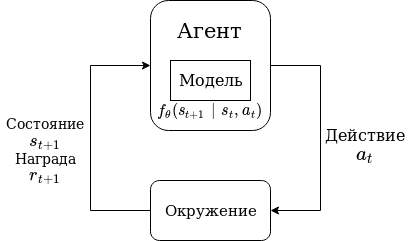
\includegraphics[height=5.5cm]{img/MBRL_ru.png}
    \caption{Обучение с подкреплением на основе модели}
    \label{fig:my_label}
\end{figure}
Таким образом, обучение прямой динамики является задачей подбора аппроксимации $\tilde{f}$ истинной переходной функции,учитывая измерения $\mathcal{D}=\{(s_n,a_n), s_{n+1}\}_{n=1}^N$ из реальной системы.\\

Обучившись динамическую модель $\tilde{f}$, мы можем использовать ее для прогнозирования распределения по траекториям состояний, возникающих в результате применения последовательности действий. Вычисляя ожидаемое вознаграждение по траекториям состояний, мы можем оценить несколько возможных последовательностей действий и выбрать оптимальную последовательность действий для использования.\\

\begin{algorithm}[H]
\SetAlgoLined
\DontPrintSemicolon
\caption{Обучение с подкреплением на основе модели}
Run a random policy;\\
Collect data $\mathcal{D}=\{(s_n,a_n), s_{n+1}\}_{n=1}^N$;\\
\For{number of iterations}{
compute the loss $\sum_i ||f_\theta(s_i,a_i)-s_{i+1}||$;\\
learn the dynamical model $f_\theta(s_t,a_t)$ by minimizing the loss;\\
\For{plan horizon}{
plan through  $f_\theta(s_t,a_t)$ to choose a sequence of actions $U^*(t)$;\\
execute the actions $U^*(t)$;\\
observe the resulting data $\{(s_t,a_t, s_{n+1})_j\}$;\\
append data $\{(s_t,a_t, s_{n+1})_j\}$ to $\mathcal{D}$;
}
}
\end{algorithm}

\subsection{Ансамбль нейронных сетей\\
Ensemble Neural Networks (ENN)}
В обучении c подкреплением на основе моделей мы должны выбрать класс моделей для прогнозирования динамики задачи (неизвестная динамическая функция). Этот выбор имеет решающее значение для алгоритмов обучения подкреплению на основе моделей, поскольку даже небольшое смещение может существенно повлиять на качество соответствующего контроллера.\\

Задача состоит в том, чтобы выбрать модель, которая может хорошо работать в режимах низких и высоких данных, т. е. на ранних стадиях обучения данные недостаточны, а высокоэкспрессивные аппроксиматоры функций могут быть переобучен. На более поздних стадиях обучения данные многочисленны, и в случае системы со сложной динамикой простые аппроксиматоры функций могут быть недостаточно недообучение.\\
\newpage
Нам нужна модель, которая может справиться с двумя типами неопределенности:
\begin{enumerate}
    \item Алеаторическая неопределенность; возникает из присущей системе стохастичности, например, шума наблюдения и шума процесса.
\item Эпистемическая неопределенность; соответствует субъективной неопределенности относительно функции динамики, из-за отсутствия достаточных данных, чтобы однозначно определить основную систему точно.
\end{enumerate}

Первый тип неопределенности может быть захвачен путем вывода параметров параметризованного распределения (математическое ожидание $\mu$ и ковариация $\Sigma$); для этого мы можем использовать параметризацию $\hat{p}_\theta(s'|s, a)=\mathcal{N}(\hat{f}_\theta(s,a),\Sigma)$.
Математическое ожидание $\hat{f}_\theta (s,a)$ задается нейронной сетью, и ковариация $\Sigma$ условного гауссовского распределения может быть обучена (или для простоты установить постоянное значение).\\

В случае бесконечных данных второй тип неопределенности исчезает, но для набора данных маленького размера эта неопределенность влияет на точность предсказания переходов. Простой и недорогой способ справиться с этой неопределенностью-использовать ансамбль нейронных сетей, которые аппроксимируют задний $p (\theta | \mathcal{D})$ с набором моделей $E$, каждая из которых имеет параметры $\theta_i$. 
В практике, с глубокими моделями нам нужно просто инициализировать параметры каждой модели $\theta_i$ с другой случайной инициализацией $\theta_i^0$ и использовать разные пакеты данных $D_i$ на каждом шаге обучения.

\begin{figure}[H]
    \centering
    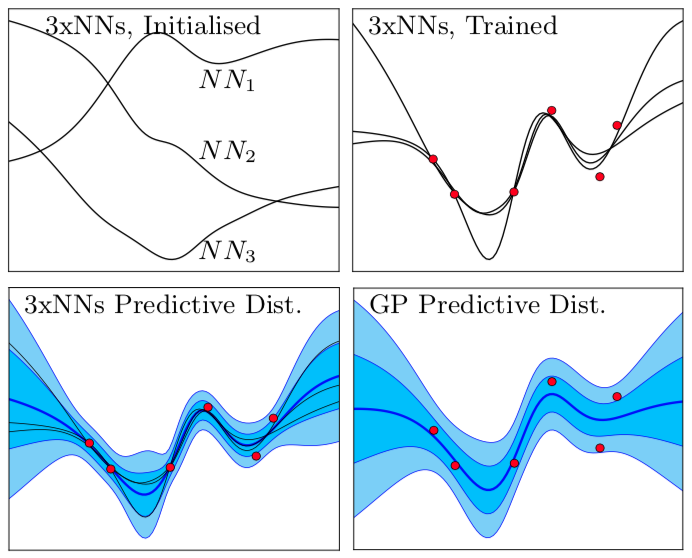
\includegraphics[height=6cm]{img/ensemble_intro.png}
    \caption{Предсказания неопределенности с ансамблю нейронных сетей}
    \label{fig:my_label}
\end{figure}

Чтобы избежать переобучения нейронных сетей, мы будем использовать метод регуляризации, называемый распадом весов.  Идея заключается в том, наказывать большие веса и эффективно ограничивать свободу в модели. Добавляя новый термин к функции стоимости, т. е.:
$$w_{я-1} \leftarrow w_i - \eta \frac{\delta E} {\delta w_i} - \eta \lambda w_i$$

Алгоритм после добавления идеи ансамбля нейронных сетей\\

\begin{algorithm}[H]
\SetAlgoLined
\DontPrintSemicolon
\caption{Обучение с ансамблю нейронных сетей}
Initialize E neural network with different random initialization $\theta_i^0$;
Run a random policy;\\
Collect data $\mathcal{D}=\{(s_n,a_n), s_{n+1}\}_{n=1}^N$\\
\For{number of iterations}{
collect $E$ datasets $\mathcal{D}_i$ by sampling N time (with replacement) from $\mathcal{D}$, $N=size(\mathcal{D})$\\
train each of the E neural network using one of datasets $\mathcal{D}_i$\\
with loss $\sum_i ||(f_\theta)_i(s_i,a_i)-s_{i+1}||$\\
\For{plan horizon}{
compute the predictive probability distribution
$$f_\theta(s_t,a_t)=\frac{1}{E}\sum_{i=1}^E (f_\theta)_i(s_t,a_t)$$\\
plan through  $f_\theta(s_t,a_t)$ to choose a sequence of actions $U^*(t)$\\
execute the actions $U^*(t)$\\
observe the resulting data $\{(s_t,a_t, s_{n+1})_j\}$\\
append data $\{(s_t,a_t, s_{t+1})_j\}$ to $\mathcal{D}$
}
}
\end{algorithm}

\newpage
\subsection{Максимизация перекрестной энтропии\\
Cross-Entropy maximization (CEM)}
Максимизация перекрестной энтропии CEM - это алгоритм стохастической оптимизации без градиента (на основе методов Monte Carlo). Мы будем использовать его в качестве оптимизатора для модельного прогностического контроллера, который будет выполнять часть планирования обучения с подкреплением на основе модели. \\

Чтобы понять CEM, мы начнаем с самого простого метода оптимизации без градиента, который называется Random-shooting. Оптимизатор Random-shooting генерирует N независимых случайных последовательностей действий ${A_0,..,A_n}$, где каждая последовательность $A_i={a_0^i, ...., a_{H-1}^i}$ имеет длину действия H.\\

Учитывая функцию вознаграждения $r(s, a)$, определяющую задачу, и учитывая прогнозы будущего состояния $\hat{s}_{t+1}=f_\theta (\hat{s}_t, a_t)+\hat{s}_t$ из обученной динамической модели $f_\theta$, оптимальная последовательность действий $A_i^*$ выбирается соответствующей последовательности с наибольшим прогнозируемым вознаграждением :
$$i^*=\argmax_i R_i=\argmax_i \sum_{t'=t}^{t+H-1}r(\hat{s}_{t'},a_{t'}^i)$$

Этот подход имеет свои недостатки: он плохо работать с большими размерами для горизонта планирования, так и пространства действий, и часто оказывается недостаточным для достижения высокой производительности задачи, поскольку последовательность действий, отобранных случайным образом, часто не приводит к значимому поведению.\\

Чтобы решить эти проблемы, CEM начинает как подход Random-shooting, но затем делает выборку для нескольких итераций $m \in {0,.., M}$ на каждом временном шаге. Для обновления и уточнения среднего значения и дисперсии выборочного распределения для следующей итерации используются топовые последовательности действий с наивысшим баллом J из каждой итерации:
$$A_i=\{a_0^i, .. a_{H-1}^i\};  a_t ^ i \sim \mathcal {N} (\mu_t ^ m, \Sigma_t ^ m)$$
$$A_{elites} =sort(A_i) [:J]$$
\newpage
$$\mu_t^{m+1}=\alpha *mean(A_{elites})+(1-\alpha)* \mu_t^m$$
$$\Sigma_t^{m+1}=\alpha * var(A_{elites})+(1-\alpha) *\Sigma_t^m$$
После M итераций выбираются оптимальные действия, которые являются результирующим средним распределением действий.\\

\begin{algorithm}[H]
\SetAlgoLined
\DontPrintSemicolon
\caption{Максимизация перекрестной энтропии CEM}
Initialize the mean $\mu$ and variance $\Sigma$\\
define variance thresholds $var_{min}$\\
determine the number of elites j\\
\While{$i<$num of iterations or max(variance)<$var_{min}$}{
draw action samples from a truncated norm distribution $a_i \sim \mathcal{N}(\mu_i,\Sigma_i)$\\
collect the samples in $A_i$\\
evaluate the generated samples (computing their costs)\\
sort the action sets according to their cost
$$sorted\_A=argsort(cost(A_i))$$
$$A_{elites}=sorted\_A[:j]$$\\
update the mean and variance
$$\mu_{i+1}=\alpha *mean(A_{elites})+(1-\alpha)* \mu_i $$
$$\Sigma_{i+1}=\alpha * var(A_{elites})+(1-\alpha) *\Sigma_i $$\\
i=i+1
}
\end{algorithm}

\newpage
\subsection{Траектория отбор проб - распространение состояния}
Вычисление стоимости действий является существенным этапом максимизации перекрестной энтропии, для этого мы должны спрогнозировать результирующее состояние применения каждого действия, формируя траекторию состояний для каждого набора действий.\\

Чтобы предсказать возможные вероятные траектории состояний, мы должны использовать нашу обученную модель (которая представляет собой ансамбль нейронных сетей), и ее свойство в учитывании неопределенности перехода.\\

Лучший способ сделать это-создать$ P $ частицы из текущего состояния, и каждая частица затем будет распространяться по нашей обученной модели:
$$s_{t+1}^p \sim \tilde{f}_\theta (s_t^p, a_t) ; s_{t=0}^p = s_0$$

Поскольку у нас есть ансамбль нейронных сетей, идея распространения частицы лучше всего реализуется путем выбора одной нейронной сети из ансамбля и распространения состоянии с помощью этой нейронной сети. \\

Это означает, что мы назначаем каждой частице одну из нейронных сетей нашего ансамбля и используем эту нейронную сеть для предсказания следующего состояния при применении действия.
$$s_{t+1}^p \sim \tilde{f}_{\theta_p}(s_t^p,a_t)$$

\begin{figure}[H]
    \centering
    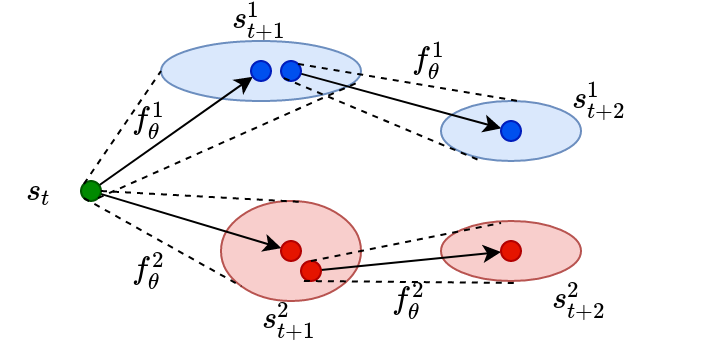
\includegraphics[height=6.5cm]{img/state_prob(1).png}
    \caption{Pаспространение состояния}
    \label{fig:my_label}
\end{figure}
\newpage
\subsection{Полный алгоритм}
Поскольку у нас есть все компоненты алгоритма, мы можем сформировать система упраиления на основане обучении следующим образом:
\begin{algorithm}
\SetAlgoLined
\DontPrintSemicolon
\caption{MPC на основе обучения с подкреплением простой}
Initialize data $\mathcal{D}$ with a random controller for one trial\\
\For{trial k=1 to K}{
Train the ensemble model with the data $\mathcal{D}$\\
\For{time t=0 to Task horizon H}{
\For{actions sampled using CEM $a_{t:t+H}$ to $N\_samples$}{
propagate state particles $s_\tau^p$ using trajectory sampling method and the trained ensemble\\
evaluate actions as $\sum_{\tau=t}^{t+H} \frac{1}{P}\sum_{p=1}^P r(s_\tau^p,a_\tau)$\\
update CEM distribution\\
}
execute the first action $a_t^*$ from optimal actions $a_{t:t+H}^*$
record the outcome: $\mathcal{D} \leftarrow \mathcal{D} \cup {s_t,a_t^*,s_t+1}$
}
}
\end{algorithm}

\begin{figure}[H]
    \centering
    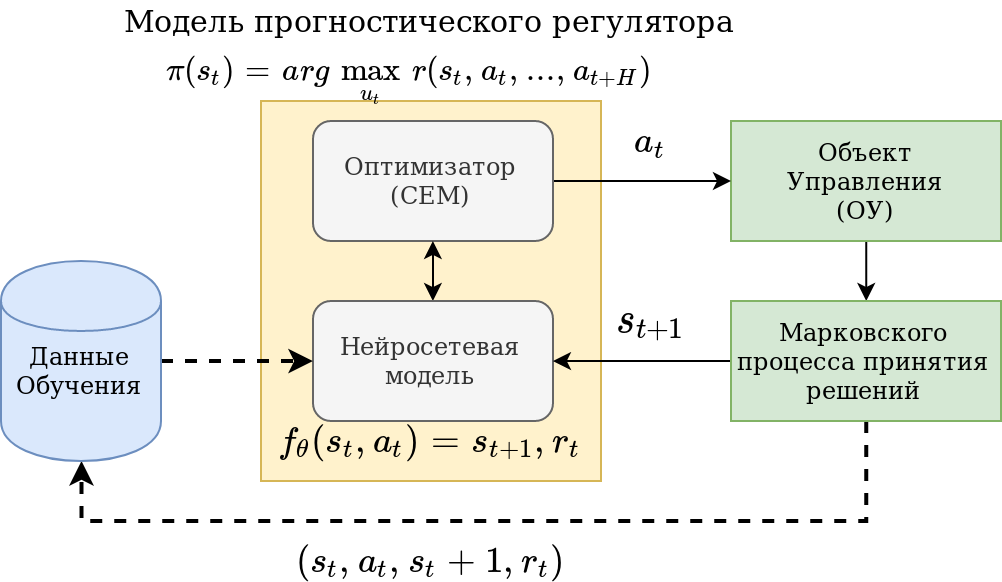
\includegraphics[width=\textwidth]{img/mpc_ru.png}
    \caption{MPC на основе обучения с подкреплением}
    \label{fig:my_label}
\end{figure}

\begin{algorithm}
\SetAlgoLined
\DontPrintSemicolon
\caption{MPC на основе обучения с подкреплением полная}
Initialize E neural network with different random initialization $\theta_i^0$\\
Initialize the mean $\mu$ and variance $\Sigma$\\
define variance thresholds $var_{min}$\\
determine the number of elites $j$\\
determine the number of particles $P$\\
Run a random controller for one trial\\
Collect data $\mathcal{D}=\{s_t,a_t,s_{t+1},r_t\}$\\
\For{number of trials}{
collect $E$ datasets $\mathcal{D}_i$ by sampling N time from $\mathcal{D}$\\
train each of the E neural network using one of datasets $\mathcal{D}_i$\\
% with loss $\sum_i ||(f_\theta)_i(s_i,a_i)-s_{i+1}||$\\
\While{max(variance)<$var_{min}$ or \#iterations<threshold}{
draw action samples $a_i \sim \mathcal{N}(\mu_i,\Sigma_i)$\\
collect action sets $A_i=a_{t:t+H}$\\
\For{each action set $A_i$}{
\For{time t in range(task horizon H)}{
initialize cost=0\\
\For{action $a_i$ from $a_{t:t+H}$}{
make $P$ particles from the current state\\
assign each particle $p$ to a model $f_{\theta}^p$\\
predict the next state distribution using the model
$s_{t+1}^p \sim f_{\theta}^p(s_t^p,a_t)$\\
compute the cost of the action and add it to the cost \newline
$cost_i+= \frac{1}{P}\sum_{p=1}^P r(s_\tau^p,a_t)$
}
update the cost of the action set
$cost(A_i)=cost_i$\\
save the cost to an array cost\_A\\
}
}
sort the action sets according to their cost
$sorted\_A=argsort(cost\_A)$\newline
$A_{elites}=sorted\_A[:j]$\\
update the mean and variance\\
% $$\mu_{i+1}=\alpha *mean(A_{elites})+(1-\alpha)* \mu_i $$
% $$\Sigma_{i+1}=\alpha * var(A_{elites})+(1-\alpha) *\Sigma_i $$\\
}
execute the first action $a_t^*$ from the optimal action set $A^*=A_{elites}[-1]$\\
add the output to the data set
% $$\mathcal{D} \leftarrow \mathcal{D} \cup {s_t,a_t^*,s_t+1}$$
}

\end{algorithm}
\newpage
\subsection{Реализация алгоритма}
Реализация алгоритма состоит из трех основных классов:
\begin{enumerate}
    \item Класс ENV :
В которой окружения определена как Марковский процесс принятия решений, она содержит функции init (), step(), reset ().
\item Класс ensemble :
Определяет динамическую модель нашей системы, она представляет собой ансамбль нейронных сетей.
Модель была реализована в PyTorch, где каждая нейронная сеть состоит из 4 слоев, каждый слой имеет 200 нейронов. Вход системы имеет размерность равное размерность действия плюс размерность состояния, а выход имеет размерность равно размерность состояния (выход является следующим состоянием). Выходной сигнал сети является математической ожидание распределения, а дисперсия рассчитывается как полоса вокруг математической ожидание.
\begin{python}
# network structure
self.layer0_w,self.layer0_b=
        get_w_b(ensemble_size,input_size,200)
self.layer1_w, self.layer1_b = 
        get_w_b(ensemble_size, 200, 200)
self.layer2_w, self.layer2_b = 
        get_w_b(ensemble_size, 200, 200)
self.layer3_w, self.layer3_b = 
        get_w_b(ensemble_size, 200, output_size)
# forward function
def forward(self, input):
    x=(input-self.inputs_mu)/self.inputs_sigma
    x=x.matmul(self.layer0_w)+self.layer0_b
    x=torch.sigmoid(x)
    x = x.matmul(self.layer1_w) + self.layer1_b
    x = torch.sigmoid(x)
    x = x.matmul(self.layer2_w) + self.layer2_b
    x = torch.sigmoid(x)
    x = x.matmul(self.layer3_w) + self.layer3_b
    mean=x[:,:,:self.output_size]
    logvar=x[:,:,:self.output_size]
    logvar=max_logvar-F.softplus(max_logvar-logvar)
    logvar=min_logvar+F.softplus(logvar-min_logvar)
    return mean,logvar
\end{python}
\item MPC class: класс, в котором реализованы все части алгоритма, и он содержит следующие методы:
\begin{enumerate}
    \item Метод инициализации (\_\_init\_\_):\\
инициализировать все параметры системы (параметры окружения, параметры модельного предсказательного регулятора , параметры ансамбля нейронных сетей, параметры максимизации кросс-энтропии, параметры распространения)
\begin{python}
# MPC parameters
self.horizon=25
self.previous_solution=np.tile(
        np.zeros(self.action_dim),[self.horizon])
# Ensemble parameters
self.E=5
self.input_size=self.action_dim+self.state_dim
self.output_size=self.state_dim
self.model=ensemble(self.E,
    self.input_size,self.output_size).to(device)
self.model.optim=torch.optim.Adam(
    self.model.parameters(),lr=0.001)
self.n_train_iter=100
self.epochs=5
self.batch_size=32
self.init_population=2000
self.has_trained=False
# CEM parameters
self.solution_dim=self.horizon*self.action_dim
self.population_size=400
self.n_elites=40
self.max_iter=5
self.alpha=0.1
self.var_min=0.001
self.action_range=[-0.2,0.2]
# propagation parameters
self.n_particles=20
self.train_in=np.array([]).reshape(0,
            self.action_dim+self.state_dim)
self.train_out=np.array([]).reshape(0,
            self.state_dim)
\end{python}
\newpage
\item rollout():\\
Запускайте политику на роботе, чтобы собрать траекторию состояний и действий. Кроме того, чтобы построить график результатов.
\item collect\_data():\\
Эта функция вызывает функцию rollout несколько раз и собирает ее выходные данные в набор данных.
\item train\_the\_model():\\
Функция для обучения динамической модели системы собирает данные, подготавливает ее к подаче ансамблю нейронных сетей путем перетасовки набора данных для каждого ансамбля, после чего запускает процедуру обучения путем вычисления оптимизации модели для минимизации стоимости (которая определяется квадратом ошибки между выходом сети и целевым выходом).
\begin{python}
idx=np.random.randint(self.train_in.shape[0],
    size=[self.E,self.train_in.shape[0]])
num_batches=int(np.ceil(idx.shape[-1]/batch_size))
for _ in range(self.epochs):
    for b in range(num_batches):
        # take a batch
        b_indx=idx[:,b*self.batch_size:
                        (b+1)*self.batch_size]
        #the loss of the uncertainty and decay
        loss=0.01*(self.model.max_logvar.sum()-
                    self.model.min_logvar.sum())
        loss+=self.model.compute_decays()
        # compute the output of the model
        mean,logvar=self.model(train_in)
        inv_var=torch.exp(-logvar)
        # compute the losses (to a scalar)
        squared_error=(mean-train_out)**2
        train_losses=squared_error*inv_var+logvar
        # the full loss
        loss+=train_losses.mean(-1).mean(-1).sum()
        # train the model
        self.model.optim.zero_grad()
        loss.backward()
        self.model.optim.step()
\end{python}
\item act(state):\\
Даст случайное действие, если модель еще не была обучена, или искать оптимальную последовательность действий с помощью оптимизатора CEM и выполняет первое действие.
\item obtain\_solution(previous\_solution):\\
Получить решение с помощью оптимизатора CEM, где матиматическое ожидание распределения является предыдущим решением, он производит выборку последовательностей действий и оценивает ее, вычисляя стоимость всех последовательностей, сортирует их и после этого обновляет матиматическое ожидание и дисперсию распределения. Выход - это среднее значение распределения после оптимизации.\\

\begin{python}
# CEM
t=0
mean=previous_solution
var=self.init_variance
truncated_normal=truncnorm(-0.2,0.2,
    loc=np.zeros_like(mean),
    scale=np.ones_like(var))
while t<self.max_iter and 
        np.max(var)>self.var_min:
    samples=truncated_normal.rvs(
        size=[self.population_size,
                self.solution_dim])
    samples=samples*np.sqrt(var)+mean
    samples=samples.astype(np.float32)
    costs=self.propagate_to_find_costs(samples)
    sorted=samples[np.argsort(costs)]
    elites=sorted[:self.n_elites]
    new_mean=np.mean(elites,axis=0)
    new_var=np.var(elites,axis=0)
    mean=self.alpha*mean+(1-self.alpha)*new_mean
    var=self.alpha*var+(1-self.alpha)*new_var
    t+=1
return mean
\end{python}
\newpage
\item propagate\_to\_find\_cost(action\_sequences):\\
Исходя из текущего состояния системы, сделайте из нее копии, число которых равные результату умножения числа последовательностей действий на число частиц. Для каждой последовательности действий; предсказать следующее состояние для каждой частицы, используя ансамбль нейронных сетей, и вычислить стоимость для этого состояния, вычислить стоимость последовательности действий путем суммирования стоимости посещенных состояний.
\begin{python}
for t in range(self.horizon):
    current_action=action_sequences[t]
    next_state=self.predict(current_state,
                            current_action)
    cost=self.state_cost(next_state)+
            self.action_cost(current_action)
    cost=cost.view(-1,self.n_particles)
    costs+=cost
    current_state=predicted_next_state
\end{python}
\item predict(state, action):\\
учитывая состояние и действие, спрогнозируйте следующее состояние с помощью ансамбля нейронных сетей.
\item run\_the\_whole\_system():\\
после обучения модели в первый раз эта функция в каждой итерации использует MPC для сбора развертки, обработки выходных данных и обучения динамической модели на нем.
\begin{python}
if not self.has_trained:
    self.train_the_model()
for i in range(num_trials):
    states,actions,next_states,ret=self.rollout()
    input=np.concatenate([states,actions],axis=-1)
    output=np.array(next_states)-np.array(states)
    self.train_in = np.concatenate(
                   [self.train_in, input], axis=0)
    self.train_out = np.concatenate(
                 [self.train_out, output], axis=0)
    self.train_the_model()
\end{python}
\end{enumerate}
\end{enumerate}
\newpage
\subsection{Результаты}

\newpage
\section{Заключение}

\newpage
\begin{thebibliography}{9}
    \addcontentsline{toc}{section}{\refname}
    \bibitem{go} Silver, D., Huang, A., Maddison, C. J., Guez, A., Sifre, L., Van Den Driessche, G., ... & Dieleman, S. (2016). Mastering the game of Go with deep neural networks and tree search. nature, 529(7587), 484.
    \bibitem{TRPO}   J. Schulman, S. Levine, P. Moritz, M. I. Jordan, and P. Abbeel. “Trust region policy optimization”. In:CoRR, abs/1502.05477 (2015).
    \bibitem{openai_gym} G. Brockman, V. Cheung, L. Pettersson, J. Schneider, J. Schulman, J. Tang, and W. Zaremba. “OpenAI Gym”. In: arXiv preprint arXiv:1606.01540 (2016).
    \bibitem{Sutton} Richard S Sutton and Andrew G Barto. Reinforcementlearning: An introduction, volume 1. MIT press Cambridge, 1998.
    \bibitem {task} Зенкевич С. Л., Ющенко А. С. Основы управления манипуляционными роботамиб Изд-во МГТУ им. Н. Э. Баумана, 2004
    \bibitem{survey} Deisenroth M.P., Neumann G., Peters J. A survey on policy search for robotics Found. Trends Robot., 2 (1–2) (2013), pp. 1-142
    \bibitem{data-efficient} Konstantinos Chatzilygeroudis, Roberto Rama, Rituraj Kaushik, Dorian Goepp, Vassilis Vassiliades, et al.. Black-Box Data-efficient Policy Search for Robotics. IEEE/RSJ International Conference on Intelligent Robots and Systems (IROS), Sep 2017, Vancouver, Canada

\end{thebibliography}

\end{document}

\usepackage[english,russian]{babel}